%!TeX program = xelatex
\documentclass[12pt,hyperref,a4paper,UTF8]{ctexart}
\usepackage{zjureport}

\begin{document}

\cover
\thispagestyle{empty}

\newpage

\begin{abstract}
本实验设计并实现了一套基于 ESP32 与华为云的智能图书馆物联网系统。
系统以 ESP32 DevKitC 为核心控制器，
集成 MF-RC522 NFC 读卡器、
M803D条码扫描模块、
BMP280 温度传感器、
DHT11 湿度传感器、
光敏电阻、
OLED 显示屏、
RGB 指示灯和风扇执行机构，
实现图书注册、借还状态感知记录、
环境数据采集、湿度联动除湿和本地状态显示等功能。

云端侧主要使用华为云 IoTDA 完成设备接入、属性上报、设备影子查询和命令下发，
使用 OBS 对象存储保存图书档案、借还历史和阅读笔记。
需要主动访问云端接口的操作大多集成在微信小程序端完成，
包括设备影子读取、图书信息查询、OBS 文件读写、远程控制以及 AI 对话；
由于华为云 FunctionGraph 功能在升级阶段，无法申请使用，
故仅作为 ISBN 查询与命令下发的一种可选尝试方案。
补充实验中还验证了 ESP32 通过 HTTPS 直接调用 DeepSeek API 的可行性，
用于理解边缘设备接入云端 AI 服务的通信流程与资源约束。
测试结果表明，系统能够稳定完成设备、小程序与云平台之间的数据同步，
借还事件响应及时，环境监测与风扇控制逻辑有效，
具备比较完整的智能图书馆原型系统价值。
\end{abstract}

\thispagestyle{empty}

\newpage
\tableofcontents
\newpage

\section{引言}

\subsection{项目背景}

传统小型图书管理通常依赖人工登记或单次扫码，无法自然记录图书取放状态，也缺少环境监测、远程查看和阅读过程数据的记录分析。随着物联网、云平台和移动端应用的发展，可以将图书标签识别、传感器采集、云端同步和移动端交互组合起来，构建低成本、可扩展的智能图书馆系统。

本项目选择“智能图书馆”作为综合实验对象，原因在于该场景同时包含感知、通信、控制、云端服务和用户交互：图书本身需要身份识别，书架环境需要实时监测，借还状态需要跨端同步，用户还希望通过手机查看书架状态并记录阅读想法。因此，该项目能够较完整地体现智能物联网系统设计的主要环节。

\subsection{设计目标}

系统设计目标如下：

\begin{enumerate}
    \item 使用 NFC 标签和条码扫描实现图书注册与身份绑定；
    \item 通过 ESP32 采集温度、湿度、光照等环境信息，并上报至华为云 IoTDA；
    \item 检测图书借出和归还事件，维护本地图书状态与云端状态；
    \item 通过微信小程序展示环境数据、藏书统计、借还历史和设备状态；
    \item 支持远程下发风扇控制和图书信息更新命令；
    \item 使用 OBS 保存图书 JSON 档案、阅读时长、借还历史和读书笔记；
    \item 集成 AI 对话能力，根据书架知识库回答图书和设备相关问题。
\end{enumerate}

\section{系统总体设计}

\subsection{总体架构}

系统采用典型的物联网三层架构：感知层、网络/平台层和应用层。

\begin{itemize}
    \item \textbf{感知层}：由 ESP32、RC522、条码扫描模块、BMP280、DHT11、光敏电阻、OLED、RGB LED 和风扇组成，负责图书身份识别、环境采集、本地显示和执行控制。
    \item \textbf{网络与平台层}：ESP32 通过 WiFi 接入互联网，使用 MQTT 与华为云 IoTDA 通信；IoTDA 保存设备影子并提供命令下发能力；OBS 用于持久化保存图书数据。
    \item \textbf{应用层}：微信小程序作为用户入口，负责设备影子查询、命令下发、OBS 图书数据读写、书架展示和 AI 问答。
\end{itemize}

\subsection{系统工作原理}

系统的基本工作原理可以概括为“本地感知、边缘判断、云端同步、移动端交互”。ESP32 作为边缘节点直接连接各类传感器和执行器：一方面周期性读取温度、湿度和光照数据，另一方面监听 NFC 与条码扫描事件。对于普通环境数据，ESP32 直接通过 MQTT 上报至 IoTDA；对于图书事件，ESP32 先在本地完成 UID 查询、状态变化和阅读时长计算，再将关键信息同步到云端。微信小程序周期性读取设备影子，并在检测到新书注册、借出、归还等状态变化时，进一步调用图书信息 API 和 OBS 接口完成图书档案云端保存。

这种设计使设备端即使在短时间网络波动时也可以保留基本状态，同时把复杂的云端 API 调用和界面交互放在小程序端处理，降低了 ESP32 固件的复杂度。IoTDA 在系统中承担设备状态中转和命令通道角色，OBS 承担轻量级数据存储角色，小程序承担用户交互角色。

\subsection{数据流设计}

系统核数据流分为四类：

\begin{enumerate}
    \item \textbf{环境数据流}：ESP32 定时读取温度、湿度和光照值，通过 MQTT 属性上报写入 IoTDA 设备影子，小程序每 5 秒查询设备影子并刷新界面。
    \item \textbf{新书注册流}：用户先将 NFC 标签贴在书上，ESP32 检测到未知 UID 后进入等待扫码状态；条码扫描模块读取 ISBN 后，ESP32 将 UID 与 ISBN 绑定并上报注册事件。
    \item \textbf{图书信息补全流}：小程序检测到新书 ISBN 后调用 \texttt{data.isbn.work} 接口查询书名、作者、出版社等信息，并将结果写入 OBS，同时可通过 IoTDA 命令下发给 ESP32。FunctionGraph 也可以实现类似流程，但由于权限不足，最终未使用该方案。
    \item \textbf{借还记录流}：已注册图书再次被 NFC 检测时，ESP32 将其状态在“在架”和“借出”之间切换，并上报图书 UID、ISBN、状态、借出次数和阅读时长；小程序监听状态变化后更新 OBS 中对应图书的 JSON 文件。
\end{enumerate}
\clearpage

\section{硬件系统设计}

\subsection{硬件清单}

\begin{table}[!htbp]
    \centering
    \begin{tabular}{l|l|c}
    \hline
        模块 & 型号/说明 & 数量 \\
    \hline
        主控开发板 & ESP32 DevKitC & 1 \\
        NFC 读卡模块 & MF-RC522，13.56MHz & 1 \\
        条码扫描模块 & M803D，UART 通信 & 1 \\
        温度传感器 & BMP280，I2C 通信 & 1 \\
        湿度传感器 & DHT11，单总线通信 & 1 \\
        光照检测 & 光敏电阻分压输入 ADC & 1 \\
        显示模块 & 0.96 寸 I2C OLED，SSD1306 & 1 \\
        指示灯 & RGB LED & 1 \\
        执行机构 & 5V 直流风扇 & 1 \\
        驱动器件 & PNP 三极管及保护电路 & 1 \\
    \hline
    \end{tabular}
    \caption{主要硬件模块清单}
    \label{tab:hardware}
\end{table}

\subsection{硬件构成}

项目硬件围绕 ESP32 主控展开，输入侧包括图书识别与环境感知模块，输出侧包括显示、指示和风扇执行模块。各模块通过 SPI、UART、I2C、ADC、GPIO/PWM 等接口与 ESP32 相连，硬件构成原理如图 \ref{fig:hardware_arch} 所示。硬件构成实物图如图 \ref{fig:hardware_photo} 所示。

\begin{figure}[!htbp]
    \centering
    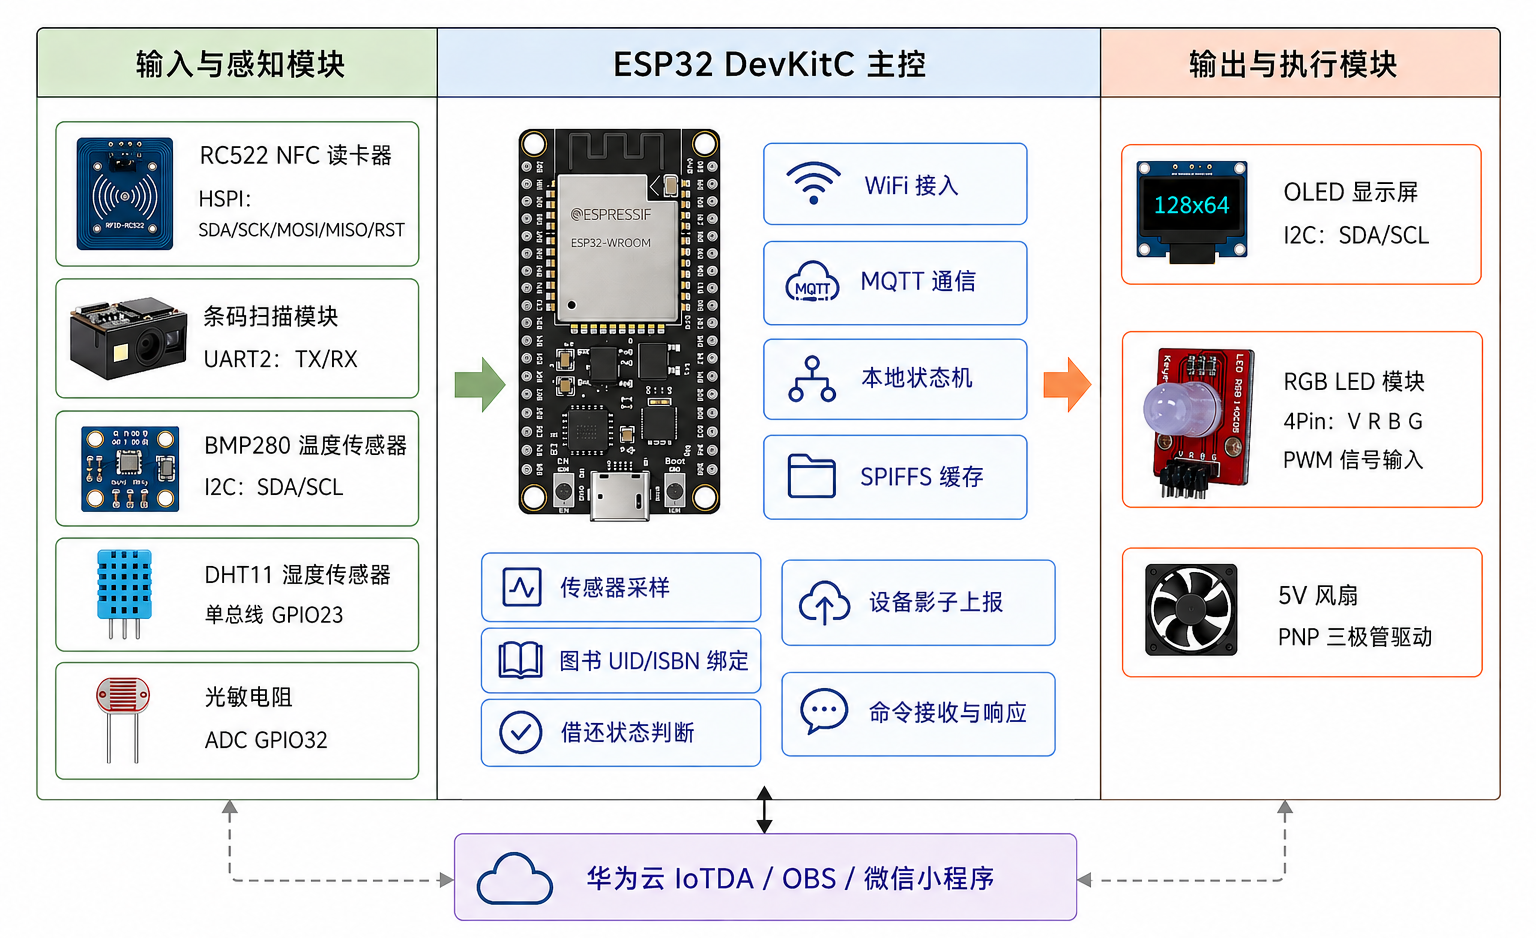
\includegraphics[width=0.8\textwidth]{figures/hardware_arch.png}
    \caption{项目硬件构成原理图}
    \label{fig:hardware_arch}
\end{figure}

\begin{figure}[!htbp]
    \centering
    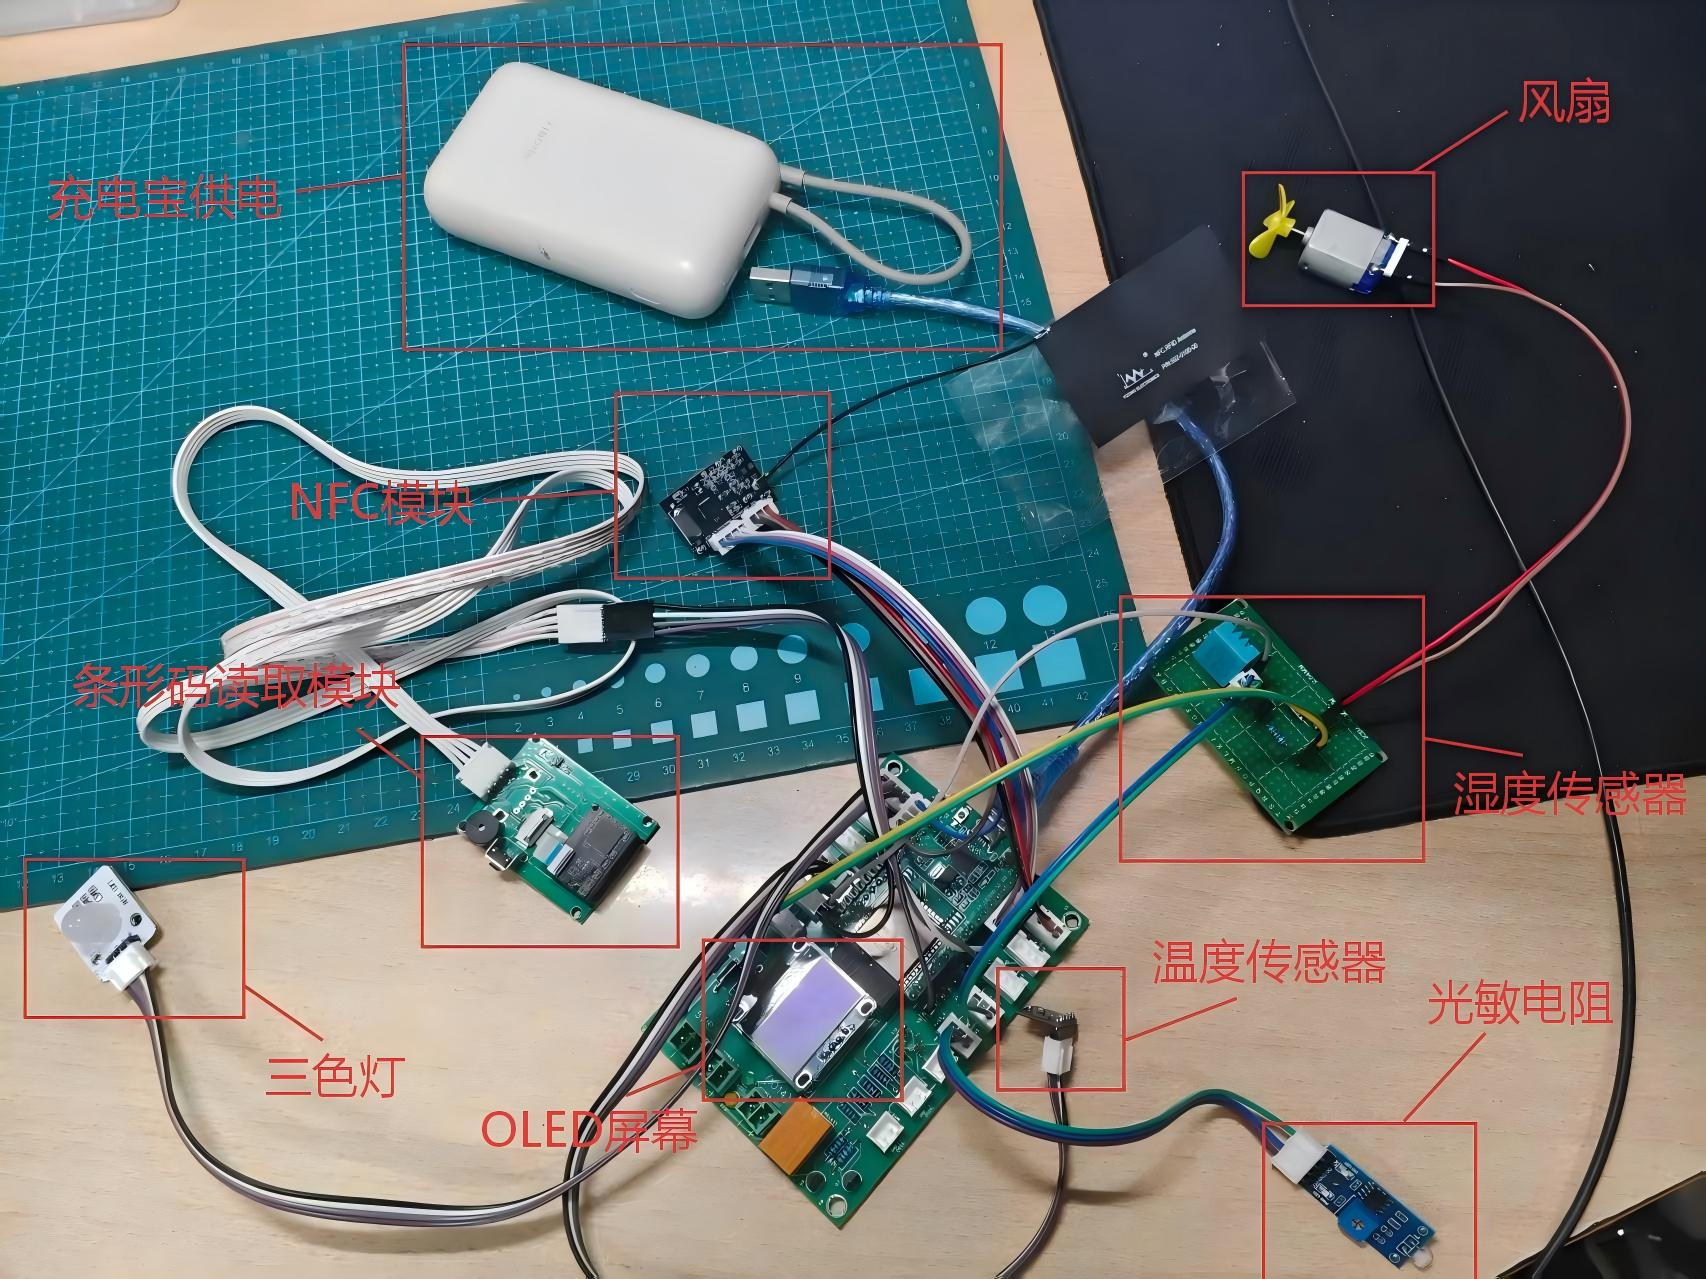
\includegraphics[width=0.8\textwidth]{figures/hardware_photo.jpg}
    \caption{项目硬件实物图}
    \label{fig:hardware_photo}
\end{figure}

\subsection{引脚分配}

系统主要引脚分配如表 \ref{tab:pins} 所示。

\begin{table}[!htbp]
    \centering
    \begin{tabular}{p{0.18\textwidth}|p{0.42\textwidth}|p{0.28\textwidth}}
    \hline
        功能模块 & ESP32 引脚 & 说明 \\
    \hline
        RC522 NFC & SDA=15, SCK=14, MOSI=13, MISO=12, RST=4 & 使用 HSPI 总线 \\
        条码扫描模块 & TX=33, RX=25 & UART2，9600bps \\
        I2C 总线 & SDA=21, SCL=22 & 连接 BMP280 与 OLED \\
        RGB LED & R=16, G=18, B=17 & PWM 输出控制颜色 \\
        光敏电阻 & GPIO32 & ADC 输入 \\
        DHT11 & GPIO23 & 湿度采集 \\
        风扇 & GPIO19 & PNP 驱动，低电平导通 \\
    \hline
    \end{tabular}
    \caption{ESP32 引脚分配}
    \label{tab:pins}
\end{table}

\subsection{图书识别模块}

图书身份由 NFC 标签 UID 与 ISBN 共同确定。NFC 标签用于日常取放识别，用户不需要每次借还书都扫描条码；ISBN 条码用于首次注册时查询书籍元数据。系统将二者绑定后形成完整图书档案：

其中 NFC 识别模块如图 \ref{fig:nfc} 所示，条码扫描模块如图 \ref{fig:barcode} 所示。

\begin{figure}[!htbp]
    \centering
    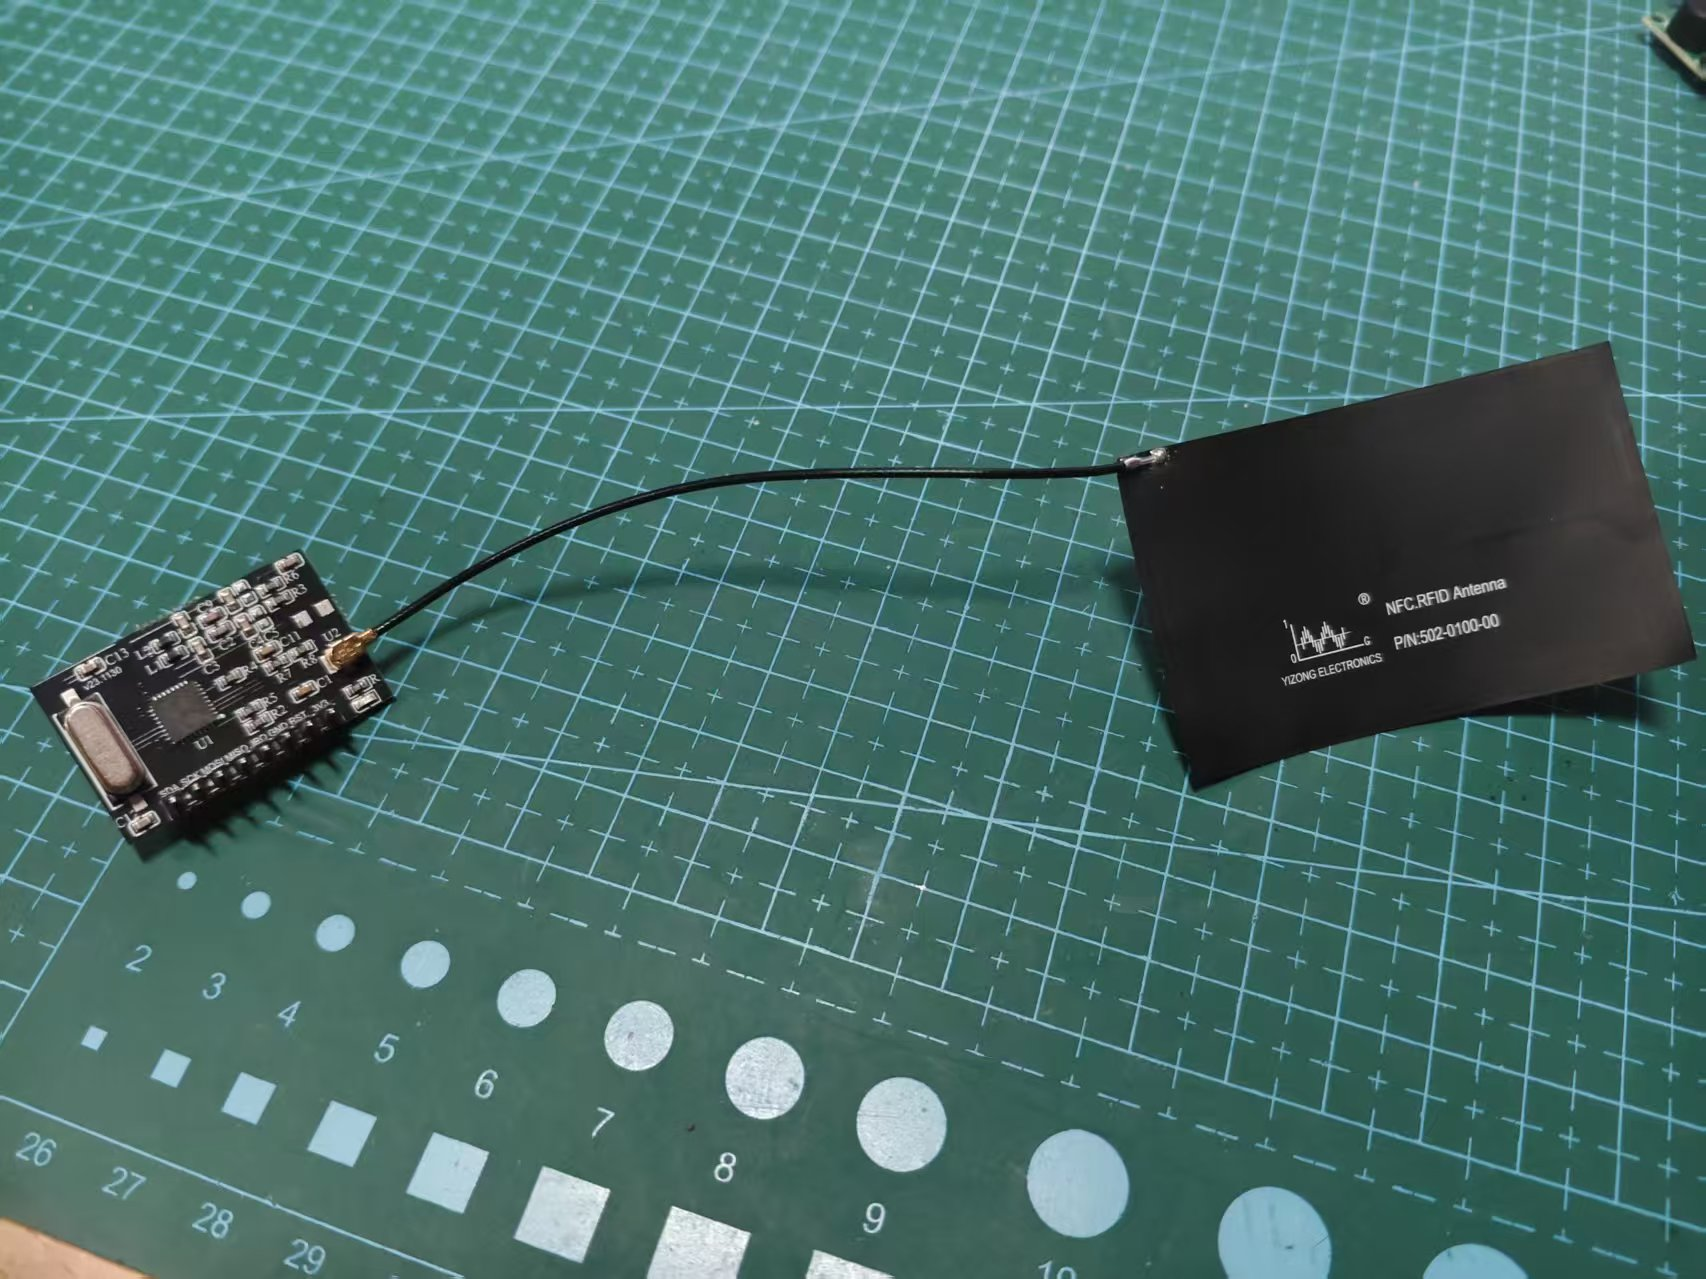
\includegraphics[width=0.4\textwidth]{figures/nfc.jpg}
    \caption{MF-RC522 NFC 模块及扩展天线}
    \label{fig:nfc}
\end{figure}

\begin{figure}[!htbp]
    \centering
    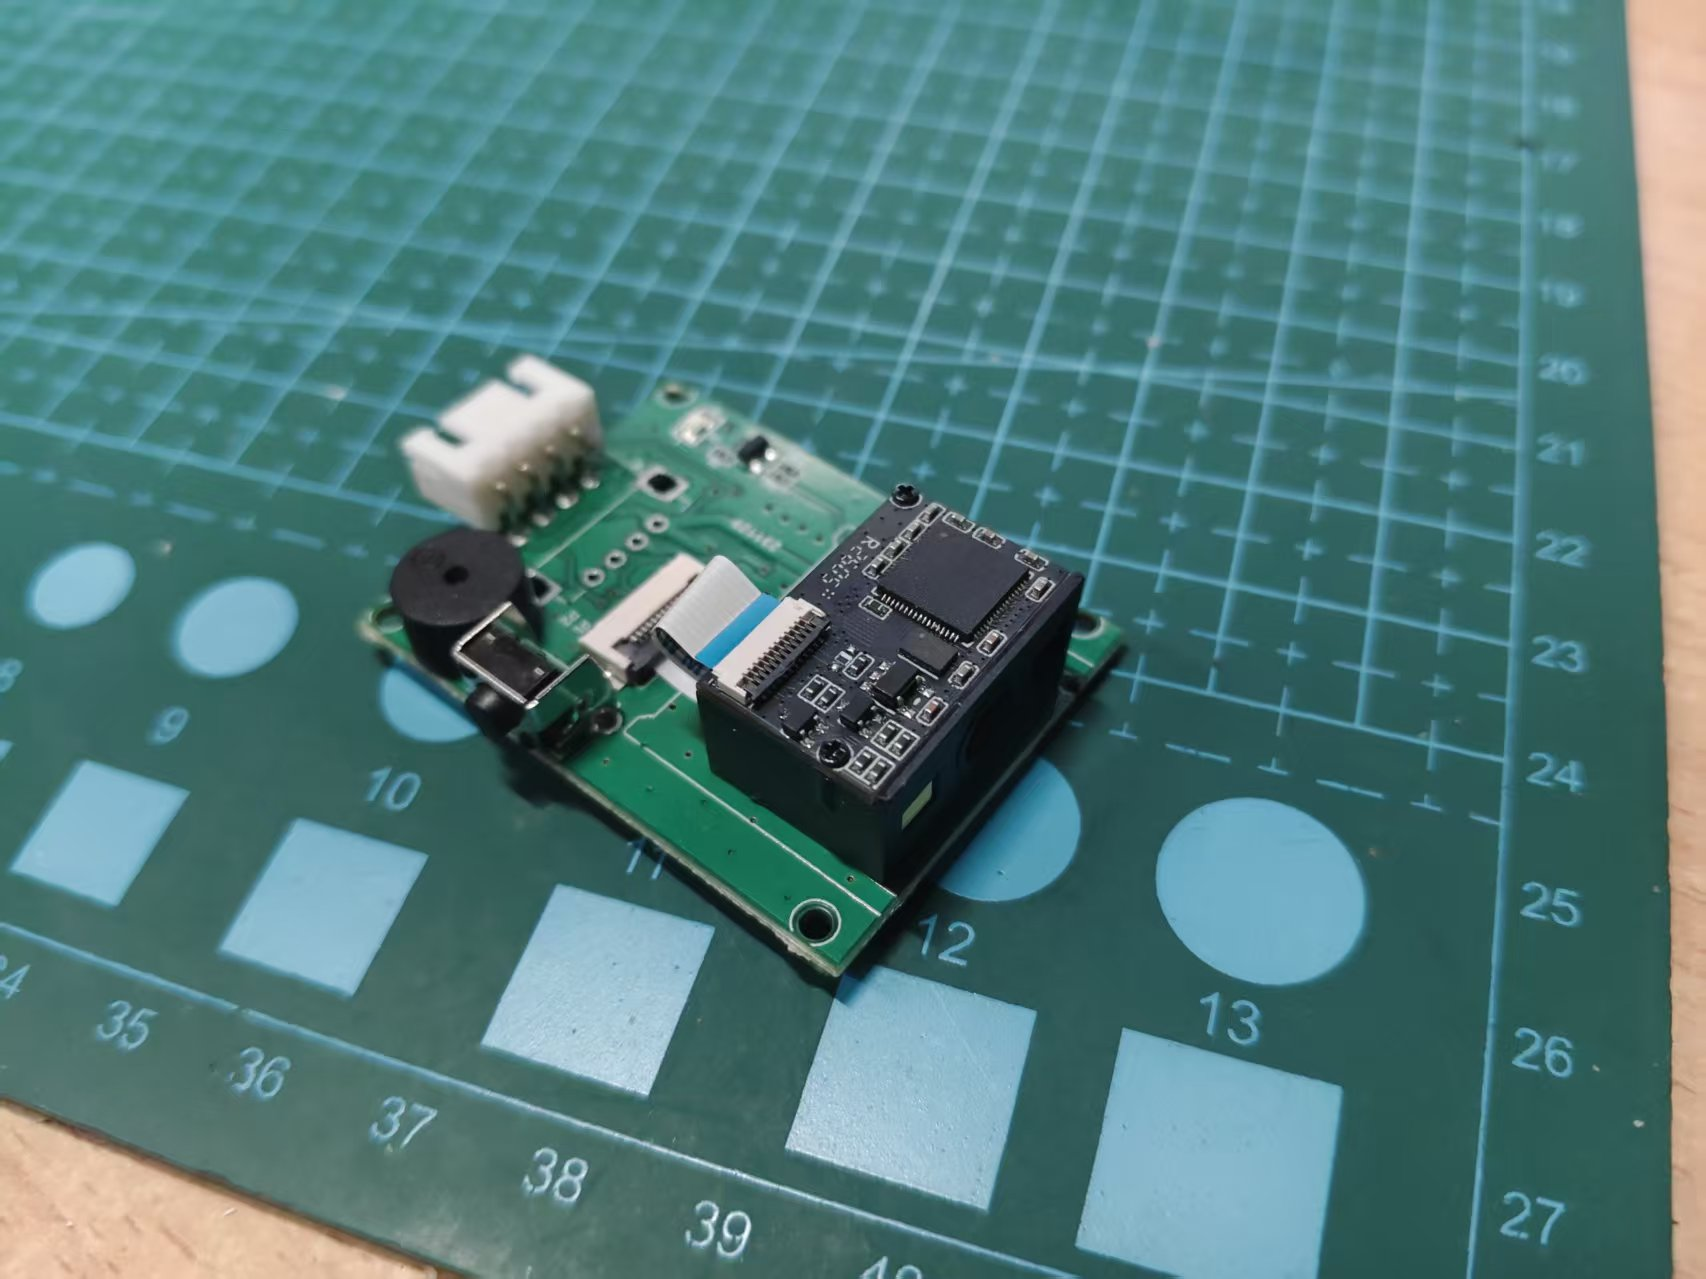
\includegraphics[width=0.4\textwidth]{figures/barcode.jpg}
    \caption{条码扫描模块}
    \label{fig:barcode}
\end{figure}

\subsection{环境监测与风扇控制}

系统使用 BMP280 读取温度，使用 DHT11 读取湿度，使用光敏电阻读取光照 ADC 值。湿度超过阈值时，风扇自动启动；用户也可以在小程序中手动开启风扇。由于风扇工作电流大于 ESP32 GPIO 可直接驱动能力，因此使用 PNP 三极管作为开关器件。最终程序中将 GPIO 低电平定义为风扇开启，高电平定义为风扇关闭，并通过 \texttt{fanManualOverride} 标志避免手动模式被自动湿度逻辑覆盖。

温度光照、三色灯以及OLED屏在课程中已经使用较多，在这里就不赘述。

读取湿度以及风扇控制部分的实物图如图 \ref{fig:fan} 所示，采用洞洞板焊接设计而成。
\begin{figure}[!htbp]
    \centering
    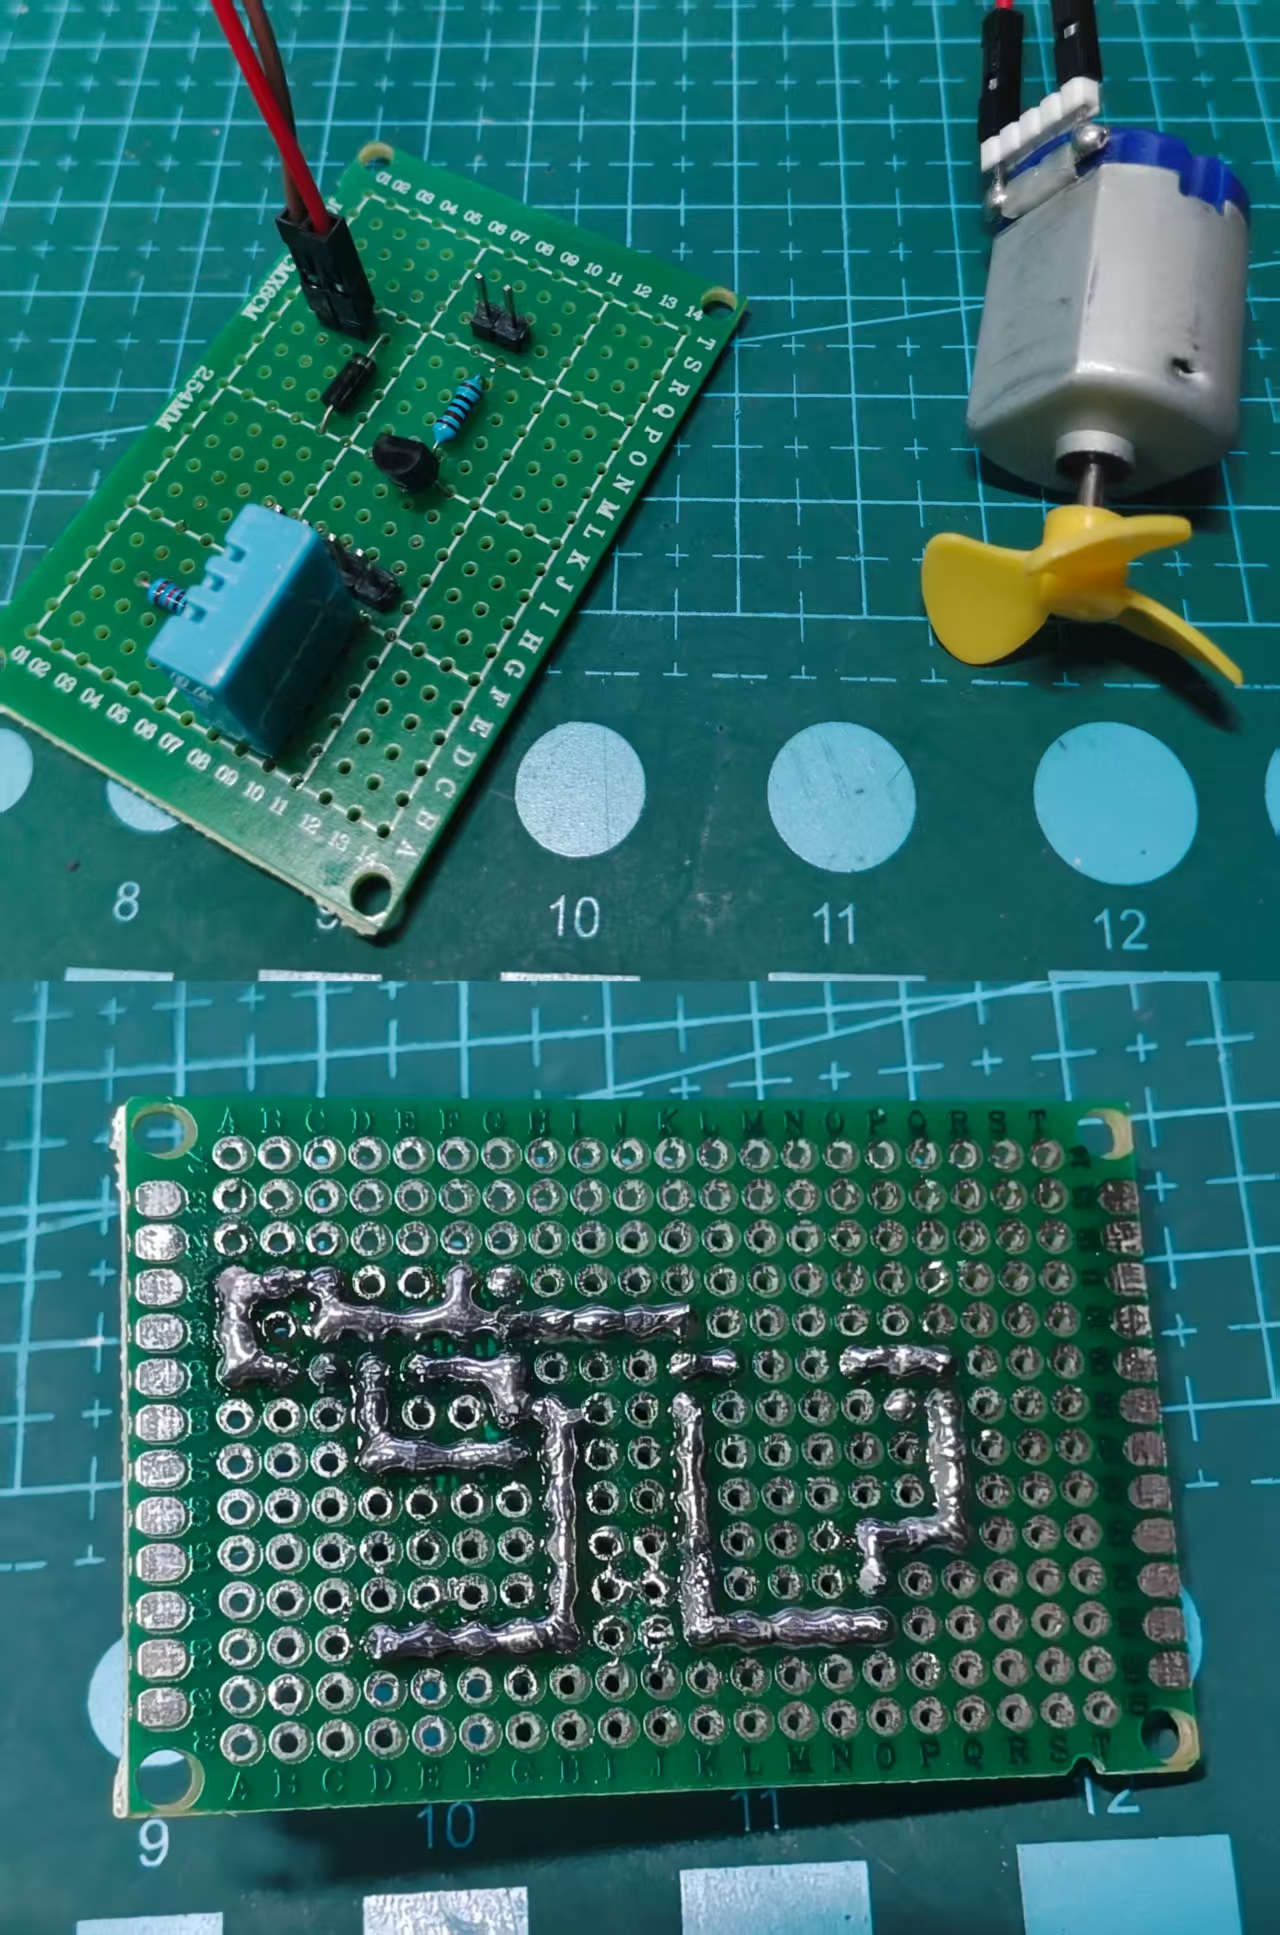
\includegraphics[width=0.4\textwidth]{figures/fan.jpg}
    \caption{风扇控制电路实物图}
    \label{fig:fan}
\end{figure}

\newpage

\section{ESP32 程序设计}

\subsection{开发环境与依赖}

程序使用 Arduino 框架开发，主要库使用如下：

\begin{itemize}
    \item \texttt{WiFi.h} 与 \texttt{PubSubClient.h}：实现 WiFi 连接和 MQTT 通信；
    \item \texttt{ArduinoJson.h}：解析云端命令和构造属性上报 JSON；
    \item \texttt{WiFiClientSecure.h} 与 \texttt{HTTPClient.h}：用于补充验证 HTTPS 请求和云端 AI API 调用；
    \item \texttt{MFRC522v2.h}：驱动 RC522 NFC 读卡模块；
    \item \texttt{HardwareSerial.h}：读取条码扫描模块输出；
    \item \texttt{SPIFFS.h}：保存本地图书缓存；
    \item \texttt{Adafruit\_BMP280.h}、\texttt{DHTesp.h}：采集温湿度；
    \item \texttt{Adafruit\_SSD1306.h}：驱动 OLED 显示屏。
\end{itemize}

\subsection{状态机设计}

固件通过 \texttt{SystemState} 状态机来维护系统状态：

\begin{lstlisting}
enum class SystemState {
  IDLE,
  AWAITING_SCAN,
  REGISTERING,
  MONITORING
};

SystemState systemState = SystemState::IDLE;
\end{lstlisting}

\begin{itemize}
    \item \texttt{IDLE}：系统正常待机，等待 NFC 事件；
    \item \texttt{AWAITING\_SCAN}：检测到未知 NFC 标签，等待用户扫描 ISBN；
    \item \texttt{REGISTERING}：预留注册处理中状态；
    \item \texttt{MONITORING}：监控已注册图书的借还状态。
\end{itemize}

当检测到未知 UID 时，系统进入 \texttt{AWAITING\_SCAN}，并启动 30 秒超时计时；若在超时前扫描到 ISBN，则完成注册并上报云端；若超时，则清空待注册 UID 并返回待机状态。

\subsection{图书借还逻辑}

由于 RC522 感应距离较短，系统采用“再次检测同一标签则改变状态”的方式判断借还。对已注册图书：

\begin{enumerate}
    \item 当前为在架状态时，再次检测判定为借出，借出次数加一，记录借出时间；
    \item 当前为借出状态时，再次检测判定为归还，根据借出时间计算本次阅读时长，并累计到图书记录；
    \item 每次状态变化后保存本地缓存，并通过 MQTT 上报图书状态。
\end{enumerate}

程序中的核心处理逻辑如下。程序先按 UID 查找图书记录，若该 UID 已存在，则翻转在架状态；若不存在，则进入等待扫码注册流程。

\begin{lstlisting}
void onBookDetected(const String& uid) {
  int idx = findBookByUID(uid);
  if (idx >= 0) {
    bool wasOnShelf = bookShelf[idx].onShelf;
    bookShelf[idx].onShelf = !wasOnShelf;
    saveBooks();

    if (wasOnShelf) {
      bookShelf[idx].lastBorrowTime = millis();
      bookShelf[idx].borrowCount++;
      reportBookStatus(uid, false);
    } else {
      unsigned long readingSec =
        (millis() - bookShelf[idx].lastBorrowTime) / 1000;
      bookShelf[idx].totalReadingSec += readingSec;
      bookShelf[idx].lastBorrowTime = 0;
      reportBookStatus(uid, true);
    }
  } else {
    pendingNFCUID = uid;
    awaitingStart = millis();
    systemState = SystemState::AWAITING_SCAN;
  }
}
\end{lstlisting}

\subsection{MQTT 属性上报与命令处理}

ESP32 使用华为云 IoTDA 标准 MQTT 主题进行通信。属性上报主题为：

\begin{lstlisting}
$oc/devices/{device_id}/sys/properties/report
\end{lstlisting}

上报内容包括温度、湿度、光照、RGB 状态、藏书总数、在架数量、借出数量和图书事件。设备订阅命令主题后可处理三类命令：

\begin{itemize}
    \item \texttt{LEDControl}：控制 RGB 指示灯颜色和开关；
    \item \texttt{FanControl}：控制风扇手动开启或交还自动控制；
    \item \texttt{deliver\_book\_info}：接收云端查询到的书名、作者、出版社和出版年份。
\end{itemize}

属性上报时，固件将传感器数据和统计数据拼接为华为云 IoTDA 要求的服务属性格式，并发布到标准主题：

\begin{lstlisting}
sprintf(props,
  "\"Temperature\":%.1f,\"Humidity\":%.0f,"
  "\"Photores\":%d,\"RED\":%d,\"GREEN\":%d,"
  "\"BLUE\":%d,\"Switch\":%d,"
  "\"BookCount\":%d,\"OnShelfCount\":%d,"
  "\"BorrowedCount\":%d,\"Time\":%ld}}]}",
  temperature, humidity, photoValue,
  rVal, gVal, bVal, deviceSwitch ? 1 : 0,
  bookCount, onShelfCount, borrowedCount, runningSec);

sprintf(msg,
  "{\"services\":[{\"service_id\":\"Env\",\"properties\":{%s",
  props);

mqtt.publish(TOPIC_PROP_REPORT, msg);
\end{lstlisting}

\subsection{ESP32 部署 DeepSeek}

在设计初期，实验中还补充验证了 ESP32 直接通过 HTTPS 调用 DeepSeek API 的方案。该方案的目的是掌握边缘设备访问云端大模型服务的基本流程，并评估其在嵌入式设备上的资源消耗和调试难点。

验证环境包括 ESP32 Dev Module、2.4GHz WiFi 网络、Arduino IDE 2.0+、ESP32 开发板库 2.0.14+、\texttt{HTTPClient} 与 \texttt{ArduinoJson}。DeepSeek 接口地址为：

\begin{lstlisting}
https://api.deepseek.com/v1/chat/completions
\end{lstlisting}

请求采用 Bearer Token 认证，主要参数包括 \texttt{model}、\texttt{messages}、\texttt{temperature} 和 \texttt{max\_tokens}。其中 \texttt{model} 使用 \texttt{deepseek-chat}，\texttt{messages} 用于组织 system/user/assistant 对话消息，\texttt{temperature} 控制回答随机性，\texttt{max\_tokens} 限制单次输出长度。

核心通信流程如下：

\begin{enumerate}
    \item ESP32 检查 WiFi 连接状态并建立 TLS 连接；
    \item 使用 HTTP POST 发送 JSON 格式请求体；
    \item 接收 DeepSeek API 返回的 JSON 响应；
    \item 使用 \texttt{ArduinoJson} 解析 \texttt{choices[0].message.content}，提取 AI 回复内容。
\end{enumerate}

代码结构如下：

\begin{lstlisting}
#include <WiFiClientSecure.h>
#include <HTTPClient.h>
#include <ArduinoJson.h>

const char* DEEPSEEK_API_KEY = "sk-xxxxxxxxxxxxxxxx";
const char* DEEPSEEK_API_URL =
  "https://api.deepseek.com/v1/chat/completions";

String askDeepSeek(const String& question) {
  WiFiClientSecure client;
  client.setInsecure();  // 实验阶段简化证书校验

  HTTPClient http;
  http.begin(client, DEEPSEEK_API_URL);
  http.addHeader("Content-Type", "application/json");
  http.addHeader("Authorization",
                 String("Bearer ") + DEEPSEEK_API_KEY);

  DynamicJsonDocument req(1024);
  req["model"] = "deepseek-chat";
  req["temperature"] = 0.7;
  req["max_tokens"] = 300;
  JsonArray messages = req.createNestedArray("messages");
  messages.createNestedObject()["role"] = "system";
  messages[0]["content"] = "你是智能图书馆助手。";
  messages.createNestedObject()["role"] = "user";
  messages[1]["content"] = question;

  String body;
  serializeJson(req, body);
  int code = http.POST(body);
  if (code != 200) return "";

  DynamicJsonDocument resp(4096);
  deserializeJson(resp, http.getString());
  return resp["choices"][0]["message"]["content"].as<String>();
}
\end{lstlisting}

测试中，ESP32 可以完成基础问答和图书推荐请求，例如根据归还图书标题生成“推荐一本类似《三体》的书”这类问题。在测试中 DeepSeek API 响应时间约 2--6 秒，单次请求 JSON 解析和响应缓存会带来约 4--6KB 的额外内存消耗。该结果说明设备端直连 AI 在原型验证中可行，但由于我们图书数据较多，使用本地部署难以将全部书籍信息写进AI的提示词当中去，相比之下小程序端调用方式更易增强上下文和用户交互体验，也更适合生成较完整的回答。

\section{华为云端服务设计}

\subsection{IoTDA 设备接入}

华为云 IoTDA 负责设备注册、MQTT 接入、设备影子存储和命令下发。物模型服务 ID 设置为 \texttt{Env}，主要属性包括 \texttt{Temperature}、\texttt{Humidity}、\texttt{Photores}、\texttt{BookCount}、\texttt{OnShelfCount}、\texttt{BorrowedCount}、\texttt{book\_uid}、\texttt{book\_isbn} 和 \texttt{book\_status} 等。实际使用时，小程序通过 IoTDA REST API 查询设备影子，并从 \texttt{shadow[0].reported.properties} 路径中获取最新属性；风扇、RGB 和图书信息下发也由小程序调用 IoTDA 命令接口完成。

Env服务的属性如图 \ref{fig:iotda} 所示。

\begin{figure}[!htbp]
    \centering
    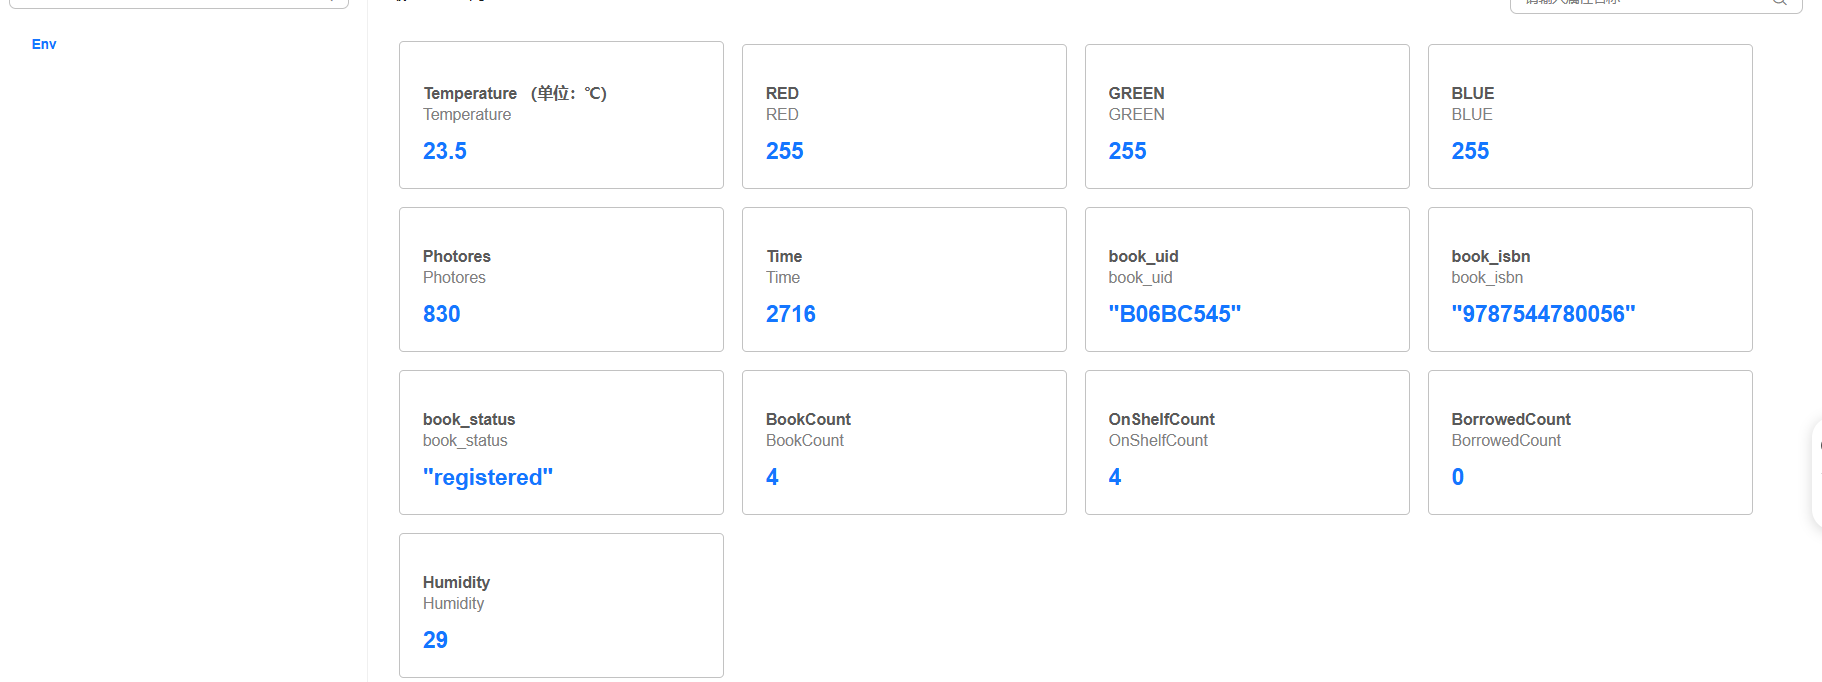
\includegraphics[width=0.8\textwidth]{figures/iotda.png}
    \caption{IoTDA 设备属性}
    \label{fig:iotda}
\end{figure}

\subsection{OBS 保存数据}

OBS 用于保存图书长期数据，每本书对应一个 JSON 文件，路径格式为：

\begin{lstlisting}
book/{isbn}.json
\end{lstlisting}

在 OBS Browser +中可以直接查看这些 JSON 文件。如\ref{fig:obs}所示。

\begin{figure}[!htbp]
    \centering
    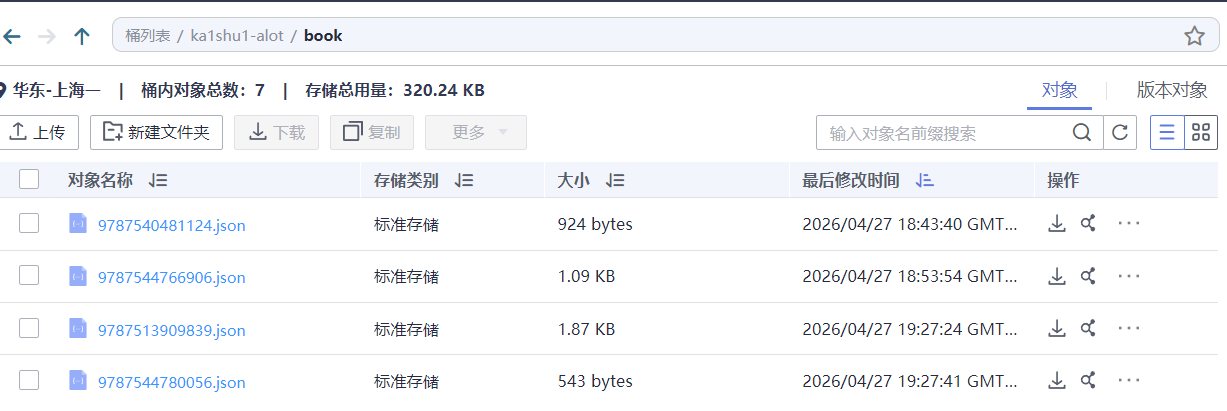
\includegraphics[width=0.8\textwidth]{figures/obs.png}
    \caption{OBS 中的图书 JSON 文件}
    \label{fig:obs}
\end{figure}

数据结构如下，以其中一本书为例，

\begin{lstlisting}
{
  "uid": "6061C645",
  "isbn": "9787540481124",
  "title": "我的前半生",
  "author": "亦舒",
  "publisher": "湖南文艺出版社",
  "currentStatus": "on_shelf",
  "borrowCount": 2,
  "totalReadingSec": 68,
  "lastBorrowTime": 0,

  "history": [
    {
      "type": "borrowed",
      "timestamp": 1777286379412,
      "typeText": "借出",
      "timeDisplay": "4月27日 18:39",
      "durationDisplay": ""
    },
    {
      "type": "borrowed",
      "timestamp": 1777286428104,
      "typeText": "借出",
      "timeDisplay": "4月27日 18:40",
      "durationDisplay": ""
    },
    {
      "type": "returned",
      "timestamp": 1777286496051,
      "durationSec": 68,
      "typeText": "归还",
      "timeDisplay": "4月27日 18:41",
      "durationDisplay": "阅读 1分钟"
    }
  ],

  "displayTitle": "我的前半生",
  "displayAuthor": "亦舒",
  "statusText": "在架",
  "statusClass": "on-shelf",
  "readingDisplay": "1m",
  "borrowCountText": "2次借出",
  "lastEventTime": "4月27日 18:41",
  "lastEventType": "归还",

  "notes": [
    {
      "content": "初读真的很暖心",
      "timestamp": 1777286620124,
      "noteTimeDisplay": "4/27 18:43"
    }
  ]
}
\end{lstlisting}

轻量化的设计便于修改查询，很适合本项目的数据储存。

\subsection{设备联动}

在云端设计了一个简单的高温报警规则：当温度超过 30℃ 时，向用户手机以及邮箱发送报警信息。效果如图 \ref{fig:alarm} 所示。

\begin{figure}[!htbp]
    \centering
    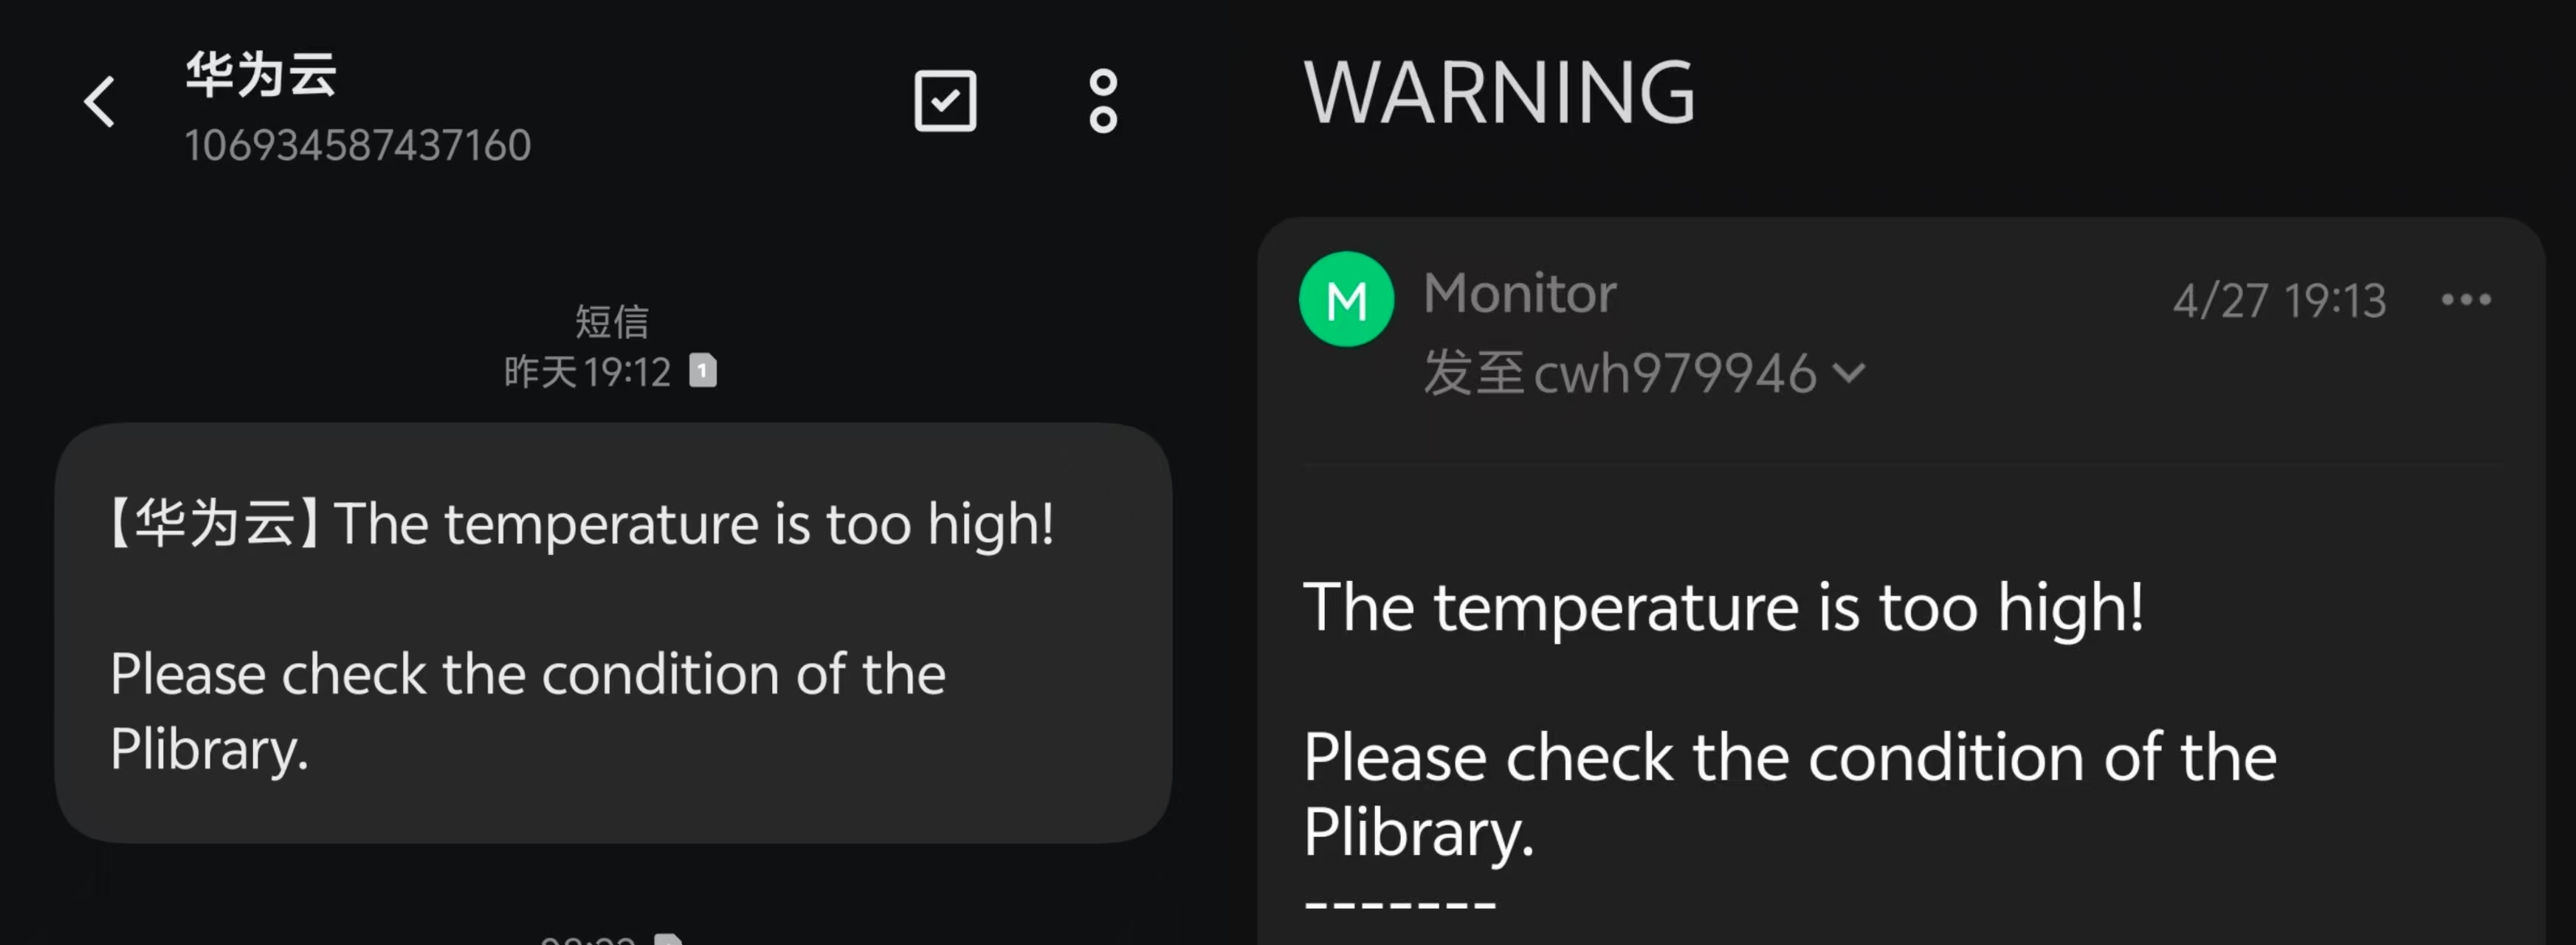
\includegraphics[width=0.8\textwidth]{figures/alarm.jpg}
    \caption{高温报警通知}
    \label{fig:alarm}
\end{figure}



\section{微信小程序设计}

\subsection{页面结构}

小程序共三个页面：

\begin{itemize}
    \item \textbf{\texttt{pages/Huawei\_IOT}}：主页面，展示环境数据、设备连接状态、藏书统计、借还动态、风扇控制、和调试日志；
    \item \textbf{\texttt{pages/bookshelf}}：书架页面，从 OBS 读取全部图书 JSON 文件，展示在架/借出状态、借出次数、阅读时长和历史记录，并支持添加阅读笔记；
    \item \textbf{\texttt{pages/ai\_chat}}：AI 对话页面，从 OBS 汇总书架知识库，调用 DeepSeek Chat API 回答用户问题。
\end{itemize}

\subsection{主页面功能}

主页面首先通过 IAM API 获取 Token，然后调用 IoTDA 设备影子接口读取设备数据。页面每 5 秒自动刷新一次，并将温度、湿度、光照、图书 UID、ISBN、借还状态和统计数量展示在界面中。用户可以在主页面手动控制风扇，以及进入书架和 AI 页面。如图 \ref{fig:main} 所示。

\begin{figure}[!htbp]
    \centering
    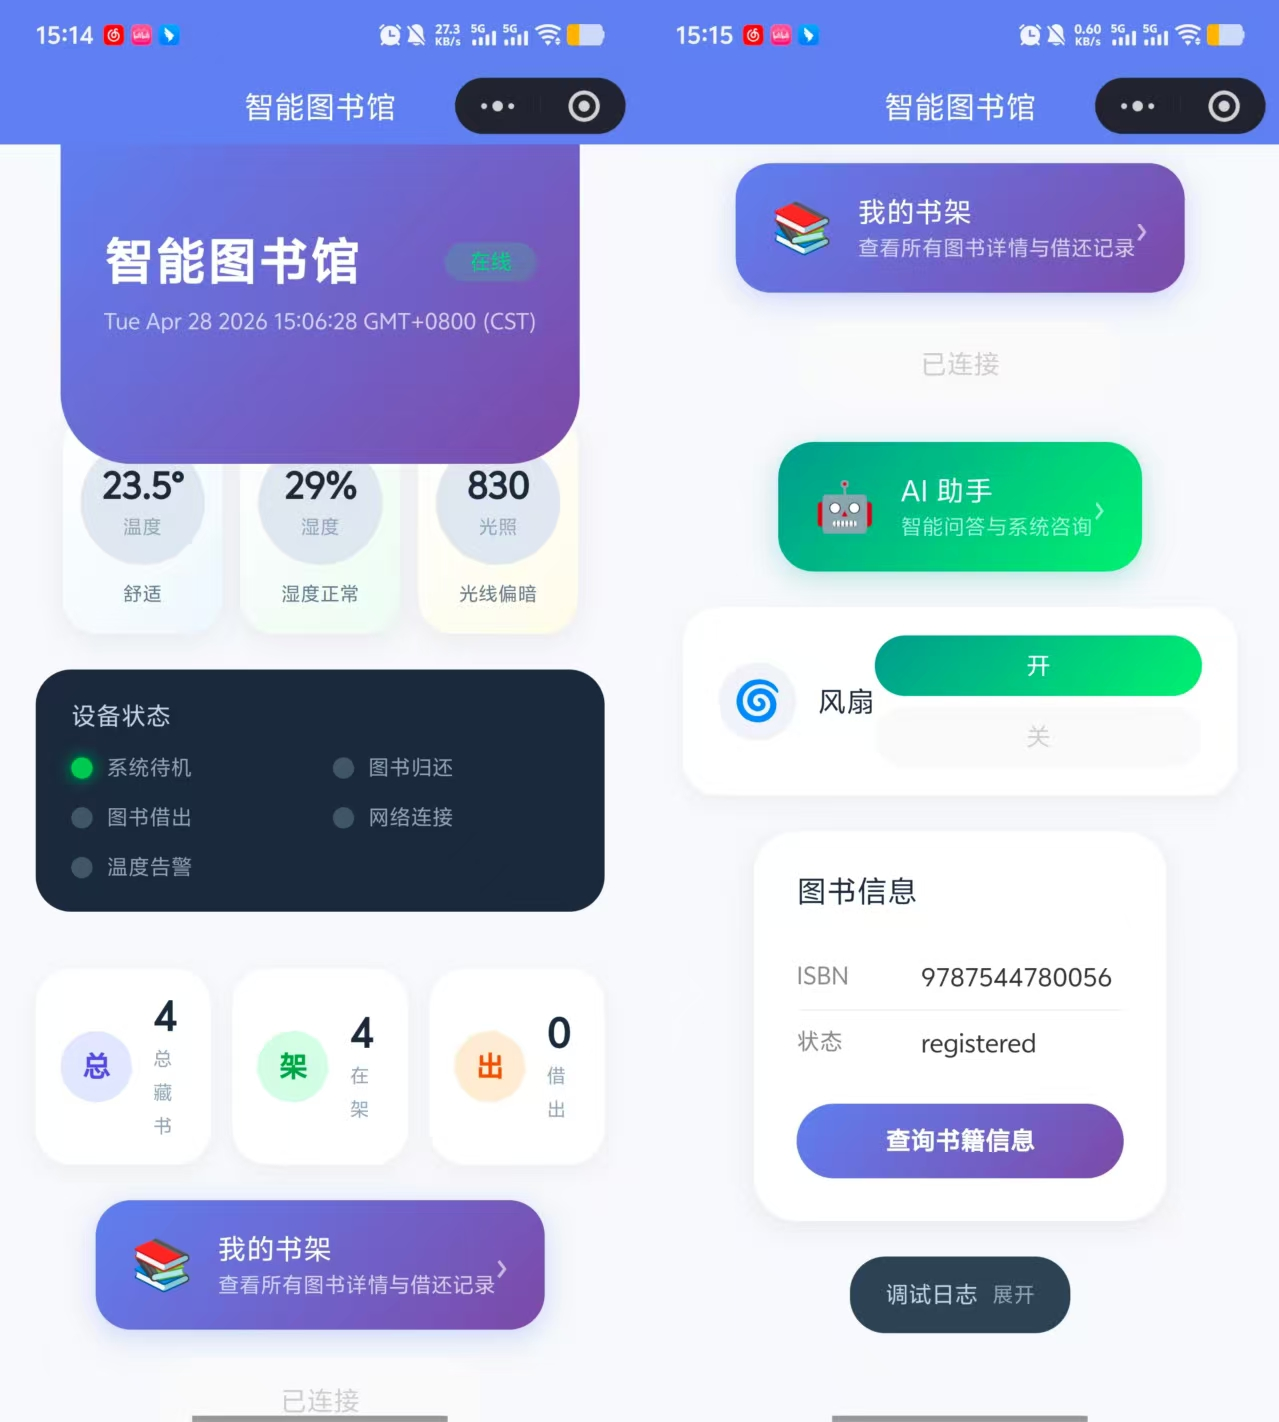
\includegraphics[width=0.8\textwidth]{figures/main.jpg}
    \caption{微信小程序主页面}
    \label{fig:main}
\end{figure}

小程序解析设备影子时，重点是从 IoTDA 返回结构中找到 reported properties。解决了早期直接读取 \texttt{reported} 导致属性为空的问题。

\begin{lstlisting}
parseShadowData: function(data) {
  var shadow = data.shadow ? data.shadow[0] : data;
  var reported = shadow.reported || shadow;
  var props = reported.properties || reported;

  this.setData({
    temperature: props.Temperature !== undefined
      ? props.Temperature.toFixed(1) + '°' : '--',
    photores: props.Photores || '--',
    humidity: props.Humidity || 0,
    bookUid: props.book_uid || props.BookUid || '',
    bookIsbn: props.book_isbn || props.BookIsbn || '',
    bookStatus: props.book_status || props.BookStatus || '',
    bookCount: props.BookCount || 0,
    onShelfCount: props.OnShelfCount || 0,
    borrowedCount: props.BorrowedCount || 0
  });
}
\end{lstlisting}

主页面按功能划分为六个区域：顶部状态栏显示系统名称、设备在线状态和最后更新时间；环境监测区以卡片形式展示温度、湿度和光照强度；LED 状态指示区展示待机、借出、归还、网络异常和温度告警等状态；藏书统计区展示总藏书量、在架数量和借出数量；最近动态区以时间线形式展示借还记录；调试日志区采用可折叠控制台，便于联调时观察 Token、设备影子和命令下发结果。

为使页面状态与硬件 RGB 指示灯保持一致，小程序端同时设计了状态灯动画规则，如表 \ref{tab:mini_led} 所示。

\begin{table}[!htbp]
    \centering
    \begin{tabular}{l|l|l}
    \hline
        状态 & 页面动画效果 & 触发条件 \\
    \hline
        系统待机 & 绿灯常亮 & 设备在线 \\
        图书归还 & 蓝灯闪烁一次 & 检测到 returned 事件 \\
        图书借出 & 红灯闪烁一次 & 检测到 taken 事件 \\
        网络异常 & 红灯慢闪 & Token 失效或请求失败 \\
        温度告警 & 红灯快闪 & 温度超过 30℃ \\
    \hline
    \end{tabular}
    \caption{小程序 LED 状态动画规则}
    \label{tab:mini_led}
\end{table}

根据图书isbn查询图书信息同样由小程序实现，调用 \texttt{data.isbn.work} API查询图书详细信息，代码如下：

\begin{lstlisting}
lookupBookByISBN: function(isbn) {
  if (!isbn) return;

  var that = this;
  that.setData({
    bookQueryStatus: 'querying',
    bookTitle: '查询中...',
    bookAuthor: '',
    bookPublisher: '',
    bookYear: '',
    result: '正在查询书籍: ' + isbn
  });
  this.addLog('查询图书: ' + isbn);

  wx.request({
    url: BOOK_API_URL,
    data: { isbn: isbn, appKey: BOOK_API_KEY },
    method: 'GET',
    success: function(res) {
      if (res.data.code === 0 && res.data.success && res.data.data) {
        var book = res.data.data;
        var year = 0;
        var pressDate = book.pressDate || '';
        var yearMatch = pressDate.match(/\d{4}/);
        if (yearMatch) year = parseInt(yearMatch[0]);

        that.setData({
          bookQueryStatus: 'success',
          bookTitle: book.bookName || '未知书名',
          bookAuthor: book.author || '未知作者',
          bookPublisher: book.press || '未知出版社',
          bookYear: year || '',
          result: '查询成功: ' + (book.bookName || isbn)
        });
        that.addLog('图书查询成功: ' + (book.bookName || isbn));

        // 查询成功后，更新 OBS 中这本书的详细信息
        that.obsUpdateBookInfo(isbn, book.bookName || '',
                               book.author || '', book.press || '');

        setTimeout(function() {
          that.sendBookInfoCommand({
            isbn: isbn,
            title: book.bookName || '',
            author: book.author || '',
            publisher: book.press || '',
            year: year
          });
        }, 500);
      } else {
        that.setData({
          bookQueryStatus: 'failed',
          bookTitle: '未找到该书籍',
          result: '未找到书籍: ' + isbn
        });
      }
    },
    fail: function(err) {
      that.setData({
        bookQueryStatus: 'failed',
        bookTitle: '查询失败',
        result: '网络错误，请重试'
      });
    }
  });
},
\end{lstlisting}

远程控制由小程序端调用 IoTDA 命令接口完成。例如风扇控制命令的程序如下：

\begin{lstlisting}
wx.request({
  url: 'https://' + iotdahttps + '/v5/iot/' +
       projectId + '/devices/' + deviceId + '/commands',
  method: 'POST',
  header: {
    'content-type': 'application/json',
    'X-Auth-Token': token
  },
  data: JSON.stringify({
    service_id: 'Env',
    command_name: 'FanControl',
    paras: { fan: on ? 'on' : 'off' }
  })
});
\end{lstlisting}

\subsection{书架与笔记功能}

书架页面通过 OBS 的 ListObjects 接口列举 \texttt{book/} 前缀下的文件。由于 OBS 列举接口返回 XML，小程序使用正则表达式提取 \texttt{Key} 和 \texttt{LastModified} 字段，再逐个读取 JSON 文件并生成书架列表。点击图书卡片可查看详情、借还历史和阅读笔记。新增笔记后，小程序将笔记写入对应 JSON 文件的 \texttt{notes} 数组，实现读书数据的存储。

\begin{lstlisting}
var regex = /<Contents>([\s\S]*?)<\/Contents>/g;
while ((match = regex.exec(res.data)) !== null) {
  var content = match[1];
  var keyMatch =
    content.match(/<Key>([\s\S]*?)<\/Key>/);
  if (keyMatch && !keyMatch[1].endsWith('/')) {
    files.push({ key: keyMatch[1] });
  }
}
\end{lstlisting}

具体实现效果如下图所示，左侧为书架总览，右侧为借还记录与读书笔记界面。

\begin{figure}[!htbp]
    \centering
    \begin{minipage}[t]{0.40\textwidth}
        \centering
        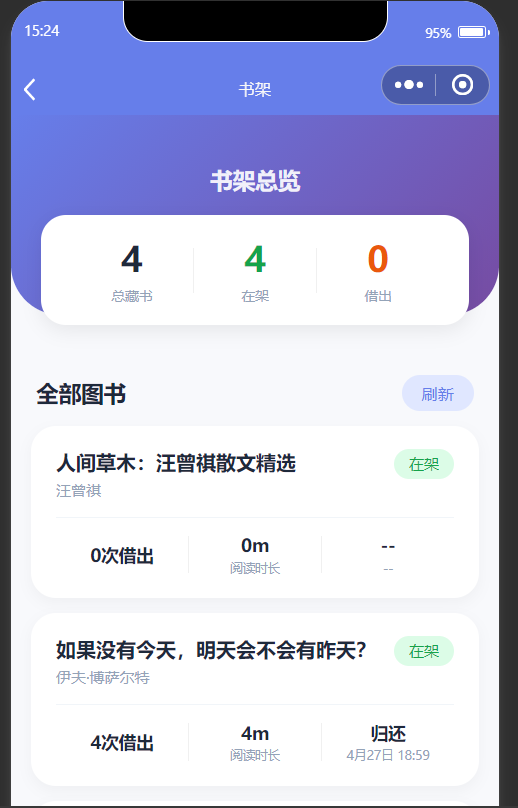
\includegraphics[width=\textwidth]{figures/bookshelf_overview.png}
        \caption{书架总览}
        \label{fig:bookshelf_overview}
    \end{minipage}
    \hfill
    \begin{minipage}[t]{0.35\textwidth}
        \centering
        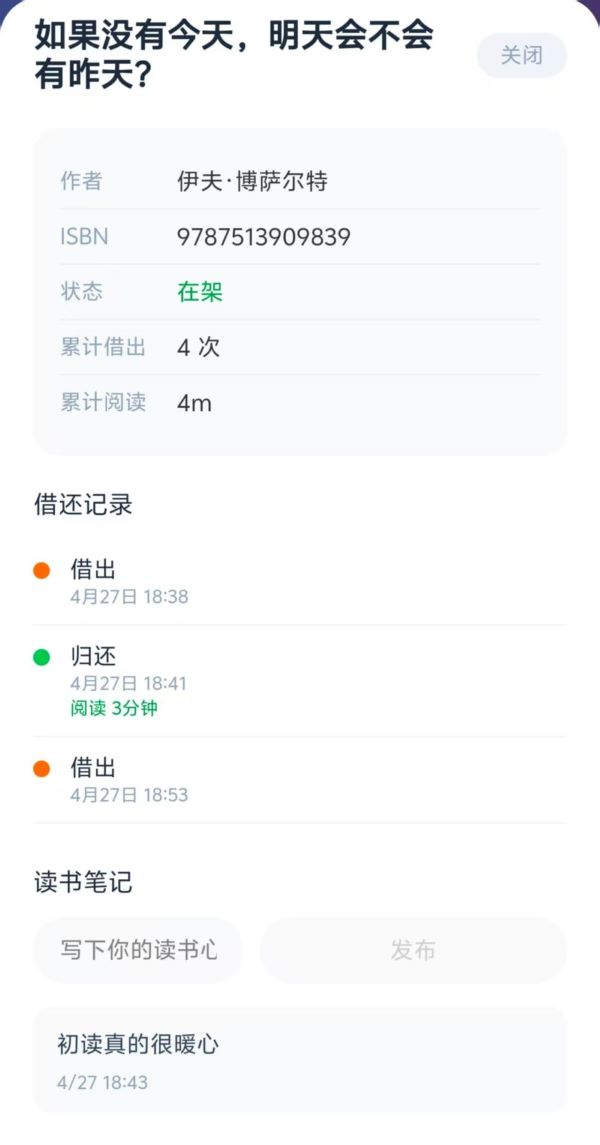
\includegraphics[width=\textwidth]{figures/borrow_return_notes.jpg}
        \caption{借还记录与读书笔记}
        \label{fig:borrow_return_notes}
    \end{minipage}
\end{figure}

\newpage

\subsection{AI 对话功能}

AI 页面启动时从 OBS 读取最多 20 本图书信息，包含书名、作者、在架状态和借出次数的书架知识库，再作为系统提示词的一部分发送给 DeepSeek Chat API。用户可以询问当前有哪些书、适合读哪本书、某本书讲了什么等问题。该功能使小程序从单纯监控界面扩展为具有一定知识服务能力的智能助手。

AI 对话功能的核心代码如下，首先通过 OBS 列举并读取图书信息构建知识库，再调用 DeepSeek API 进行问答：

\begin{lstlisting}
// pages/ai_chat/ai_chat.js

const API_KEY = '';
const API_URL = 'https://api.deepseek.com/v1/chat/completions';

// ============== DeepSeek API 调用 ==============
callDeepSeek: function(messages) {
  var that = this;
  var systemContent = '你是一个智能图书馆助手，正在回答用户关于图书馆的问题。';
  var ctx = this.data.bookContext;
  if (ctx) {
    systemContent += '书架知识库：' + ctx + '。';
  }
  var apiMsgs = [{ role: 'system', content: systemContent }];
  messages.forEach(function(m) {
    apiMsgs.push({ role: m.role, content: m.content });
  });

  wx.request({
    url: API_URL,
    method: 'POST',
    header: {
      'Content-Type': 'application/json',
      'Authorization': 'Bearer ' + API_KEY
    },
    data: {
      model: 'deepseek-chat',
      messages: apiMsgs,
      max_tokens: 600,
      temperature: 0.7
    },
    success: function(res) {
      if (res.statusCode === 200 && res.data && res.data.choices && res.data.choices[0]) {
        var reply = res.data.choices[0].message.content;
        var updated = that.data.messages;
        updated.push({ role: 'assistant', content: reply });
        that.setData({ messages: updated, thinking: false });
      } else {
        that.addError('API 响应异常');
      }
    },
    fail: function(err) {
      that.addError('网络错误: ' + (err.errMsg || ''));
    }
  });
},

\end{lstlisting}

在小程序端调用api不用受硬件算力的限制，能够给出比较完整有效的回答，示例如图\ref{fig:ai_chat_example}所示：

\begin{figure}[!htbp]
    \centering
    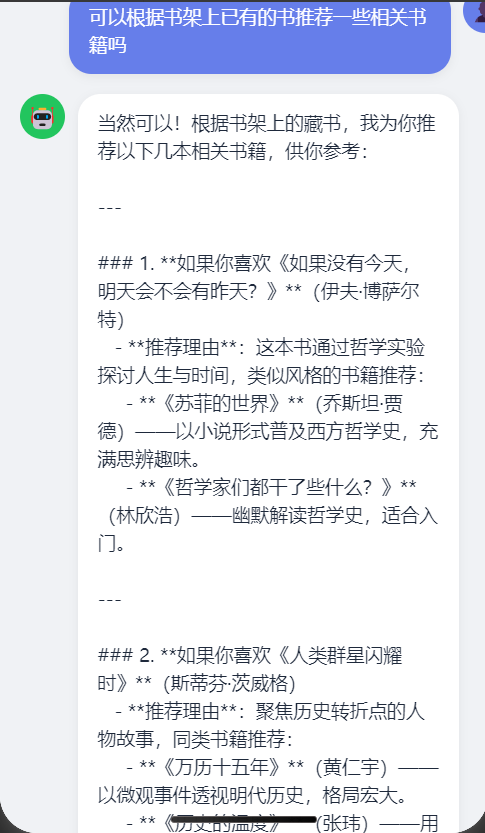
\includegraphics[width=0.8\textwidth]{figures/ai_chat_example.png}
    \caption{AI 对话示例}
    \label{fig:ai_chat_example}
\end{figure}

与 ESP32 直连 AI 的补充实验相比，小程序端方案可以更方便地组织多轮消息、拼接 OBS 书架知识库，也避免 API Key 固化在设备固件中。最终系统因此采用小程序端作为 AI 服务入口，ESP32 直连方案作为边缘 AI 通信能力验证保留在实验记录中。


\section{实验过程}

本实验按照“单模块验证、设备端集成、云端接入、小程序联调、整体测试”的顺序推进。

\begin{enumerate}
    \item \textbf{需求分析与方案确定}：首先确定智能图书馆的核心功能，包括图书身份识别、借还状态记录、环境监测、远程控制和阅读数据管理。随后确定采用 NFC 识别日常取放、条码扫描绑定 ISBN、小程序作为主要用户界面的方案。
    \item \textbf{硬件模块独立测试}：分别测试 RC522 NFC 读卡器、M803D 条码扫描模块、BMP280、DHT11、光敏电阻、OLED 和风扇驱动电路，确认各模块接线、通信接口和基本读写功能正常。
    \item \textbf{ESP32 代码集成}：在独立测试基础上整合状态机、图书缓存、借还判断、传感器采集、MQTT 上报和命令处理逻辑，使设备端能够独立完成图书事件识别和环境数据采集。
    \item \textbf{华为云 IoTDA 接入}：创建产品和设备，配置物模型属性与命令，完成 ESP32 MQTT 接入、属性上报和命令订阅。通过设备影子验证温度、湿度、光照、藏书统计等数据是否正确更新。
    \item \textbf{微信小程序开发}：开发主页面、书架页面和 AI 对话页面。主页面负责设备影子查询和命令下发，书架页面负责 OBS 图书数据展示与笔记保存，AI 页面负责基于书架知识库进行问答。
    \item \textbf{OBS 存储桶设计}：将每本书的数据保存为 OBS 中的 JSON 文件，逐步补充注册、借出、归还、阅读时长和笔记字段，并通过小程序端完成读取、更新和展示。
    \item \textbf{整体测试}：按照“新书贴 NFC 标签、扫描 ISBN、查询图书信息、借出、归还、查看书架、添加笔记、AI 问答、远程控制风扇”的流程进行完整测试，确认端、云、应用三部分能够形成闭环。
\end{enumerate}

\section{系统调试与问题解决}

项目调试过程中遇到的主要问题和解决方案如下：

\begin{enumerate}
    \item \textbf{DHT11 读取稳定性问题}：早期驱动方案在 ESP32 上出现看门狗超时的情况，后改用 \texttt{DHTesp} 库，解决了串口写入数据的问题。
    \item \textbf{设备影子解析路径错误}：IoTDA 返回数据嵌套在 shadow 数组第一项的 reported properties 中，由于实验中更改过设备影子，故读取的都是旧属性的设备影子。在找到问题后通过清楚设备影子、修正小程序解析逻辑后解决。
    \item \textbf{OBS 列举返回 XML}：小程序原本按 JSON 处理失败，后改为解析 XML 中的 \texttt{Contents} 和 \texttt{Key} 字段。
    \item \textbf{手动开启风扇控制被自动检测逻辑覆盖}：加入 \texttt{fanManualOverride} 标志，手动开启时跳过湿度自动控制。
    \item \textbf{借还事件重复写入}：小程序使用 \texttt{lastProcessedEvent} 记录最近处理的 UID 和状态组合，避免重复触发导致的 OBS 多次写入。
    \item \textbf{ESP32 HTTPS 请求失败}：直接调用 DeepSeek API 时，\texttt{HTTPClient} 曾返回连接错误。实验阶段使用 \texttt{client.setInsecure()} 跳过证书校验完成验证，正式系统应配置根证书或改由云端/小程序代理。
    \item \textbf{AI 响应 JSON 解析失败}：DeepSeek 返回内容较长时，固定 JSON 缓冲区不足，后将响应解析缓冲区增大到 4096 字节，并限制 \texttt{max\_tokens} 控制单次回复长度。
    \item \textbf{API 认证和余额问题}：当接口返回 401 或 402 时，分别检查 API Key 格式与账户额度，重新生成以 \texttt{sk-} 开头的密钥或补充额度后恢复请求。
    \item \textbf{NFC 感应距离较短以及无法检测多本书籍}：通过调整操作方式和采用状态翻转逻辑完成基本功能。
\end{enumerate}

\section{实验结果}

\subsection{功能测试视频}

已随报告一并上交，主要内容（按照视频顺序）为：

\begin{itemize}
    \item 小程序整体功能展示，包括：环境数据监控、书架整体展示、风扇控制。
    \item 图书借还流程。
    \item 图书注册流程。
    \item 湿度检测与除湿功能。
    \item 小程序远程下发发命令开启风扇。
    \item AI图书助手问答以及读书笔记。
    \item 温度警报。
\end{itemize}

\subsection{实验源代码}

已随报告一并上交。


\section{总结与展望}

\subsection{项目成果}

本项目完成了一套从硬件感知到云端平台再到移动端应用的完整智能物联网系统。系统能够通过 NFC 与 ISBN 结合完成图书注册，通过传感器采集书架环境，通过 IoTDA 实现设备状态同步和远程命令控制，通过 OBS 保存图书档案与阅读记录，并通过微信小程序和 AI 对话提供较完整的人机交互体验。同时，我们也验证了 ESP32 通过 HTTPS 直连 DeepSeek API 的可行性，进一步理解了边缘设备调用云端 AI 服务时的 TLS、JSON 解析、响应延迟和内存占用问题。相比单一的传感器采集实验，本项目更强调端云协同、数据闭环和实际应用场景。

\subsection{不足与改进方向}

后续可从以下方面继续优化：

\begin{enumerate}
    \item \textbf{个人记录}：小程序端手动输入书籍信息并下发设备，上传云端（比如有些日记本、笔记本没有条形码或者条形码不具有特殊性）
    \item \textbf{识别距离}：RC522 感应距离较短，且无法读取多个标签，此后可尝试更合适的天线、NFC 标签或其他 RFID 方案；
    \item \textbf{安全性}：为方便读写，当前 OBS 读写方案为匿名用户直接读写桶内内容。正式系统应使用签名 URL、IAM身份认证或更细粒度的权限控制；
    \item \textbf{数据一致性}：可引入数据库或云函数统一处理借还事件，减少小程序端直接写 OBS 带来的并发风险；
    \item \textbf{可视化}：可增加温湿度历史曲线、借阅趋势图和阅读时长统计；
    \item \textbf{多设备扩展}：未来可支持多个书架节点，并在云端按设备 ID 汇总不同区域的藏书状态。
\end{enumerate}

\subsection{心得体会}

这次大作业的制作还是让我收获颇丰的，之前做的实验大多有明确的过程和参考，
但这次是第一次从零开始重新创造一个系统。在这个过程中，我不仅需要设计系统架构、
选择合适的硬件和云服务，还要处理各种实际问题，比如设备间通信串口选择与设计、
数据格式转换、网络请求失败等等。这些都是之前几乎没有经历过的挑战，
但也正是这些挑战让我学到了很多实用的技能和经验。
在软件端，我重温了如何设计状态机来管理系统状态，如何使用 MQTT 协议进行设备与云端的通信，
也初步学习了爬虫原理，JSON与XML格式数据的处理与转换；
在硬件端，分配引脚并接线在初期是不小的挑战，尤其是第一次处理洞洞板上接线，
从刚开始的生疏到最后的游刃有余，变化和成长还是很大的。
同时这个大作业也是我第一个从开始到完成都使用git记录并管理的项目，给予了我更熟练的操作以及宝贵的开发经验。

通过这个项目，我更深入地理解了物联网系统中设备端、云端和应用端之间的协同工作流程，
也体会到了从硬件调试到云服务配置再到前端开发的全栈开发过程中的挑战与乐趣。
尤其是在调试过程中遇到的各种问题，让我学会了如何定位问题、分析原因并找到解决方案，
这些都是非常宝贵的经验。未来我希望能继续在物联网和智能系统领域深入学习和实践，
打造更多有趣实用的项目。

\newpage

\reference
\nocite{huawei-support}
\nocite{randomnerd-esp32-mfrc522}
\nocite{yhd-m803d-manual}
\nocite{lckfb-dht11}
\nocite{randomnerd-esp32-dht}
\nocite{espressif-devkitc-guide}
\nocite{isbn-work-api}
\nocite{ecslab-slibrary}



\appendix

\section{附录}

实验项目已开源在github仓库：\url{https://github.com/Altokra/AIoT\_project}

\end{document}


